\documentclass[a4paper, 12pt]{article}

\usepackage{cmap}
\usepackage[T2A]{fontenc}
\usepackage[utf8]{inputenc}
\usepackage{amssymb}
\usepackage{graphicx}
\graphicspath{ {./images/} }
\usepackage[english, russian]{babel}
\usepackage{mathtools}
\usepackage[top=1in, bottom=1in, left=1.25in, right=1.25in]{geometry}
\newcommand{\parag}[1]{\paragraph{#1}\mbox{}\\}

\begin{document}
\section{Определения}

\parag{1. Логические операции: конъюнкция, дизъюнкция и отрицание.}
1) \underline{Конъюнкция} - это сложное логическое выражение, которое считается истинным в том и только том случае, когда оба простых выражения являются истинными, во всех остальных случаях данное сложеное выражение ложно.

Обозначение: F = A $\land$ B.

Таблица истинности для конъюнкции:

\begin{center}
    \begin{tabular}{|c|c|c|}
        \hline
        A & B & A $\land$ B  \\
        \hline
        0 & 0 & 0  \\
         \hline
        0 & 1 & 0  \\
        \hline
        1 & 0 & 0 \\
        \hline
        1 & 1 & 1 \\
        \hline
    \end{tabular}
\end{center}

\noindent
2) \underline{Дизъюнкция} - это сложное логическое выражение, которое истинно, если хотя бы одно из простых логических выражений истинно и ложно тогда и только тогда, когда оба простых логических выраженныя ложны.

Обозначение: F = A $\vee$ B.

Таблица истинности для дизъюнкции:

\begin{center}
    \begin{tabular}{|c|c|c|}
        \hline
        A & B & A $\vee$ B  \\
        \hline
        0 & 0 & 0  \\
         \hline
        0 & 1 & 1  \\
        \hline
        1 & 0 & 1 \\
        \hline
        1 & 1 & 1 \\
        \hline
    \end{tabular}
\end{center}

\noindent
3) \underline{Отрицание}  - это сложное логическое выражение, в котором если исходное логическое выражение истинно, то результат отрицания будет ложным, и наоборот, если исходное логическое выражение ложно, то результат отрицания будет истинным.

Обозначение: F = $\neg$A

Таблица истинности для отрицания:
\begin{center}
    \begin{tabular}{|c|c|}
        \hline
        A & $\neg$A  \\
        \hline
        0 & 1  \\
         \hline
        1 & 0  \\
        \hline
    \end{tabular}
\end{center}

\parag{2. Логические операции: импликация, XOR (исключающее или) и эквивалентность.}
1) \underline{Импликация} - это сложное логическое выражение, которое истинно во всех случаях, кроме случая, когда из истины следует ложь. То есть данная логическая операция связывает два простых логических выражения, из которых первое является условием (А), а второе (В) является следствием.

Обозначение: F = A $\to$ B

Таблица истинности для импликации:

\begin{center}
    \begin{tabular}{|c|c|c|}
        \hline
        A & B & A $\to$ B  \\
        \hline
        0 & 0 & 1  \\
         \hline
        0 & 1 & 1  \\
        \hline
        1 & 0 & 0 \\
        \hline
        1 & 1 & 1 \\
        \hline
    \end{tabular}
\end{center}

2) \underline{XOR (исключающее или)} -  это сложное логическое выражение, которое является истинным тогда и только тогда, когда оба простых логических выражения имеют разную истинность.

Обозначение: F = A $\oplus$ B

Таблица истинности для исключающего или:

\begin{center}
    \begin{tabular}{|c|c|c|}
        \hline
        A & B & A $\oplus$ B  \\
        \hline
        0 & 0 & 0  \\
         \hline
        0 & 1 & 1  \\
        \hline
        1 & 0 & 1 \\
        \hline
        1 & 1 & 0 \\
        \hline
    \end{tabular}
\end{center}


3) \underline{Эквивалентность} - это сложное логическое выражение, которое является истинным тогда и только тогда, когда оба простых логических выражения имеют одинаковую истинность.

Обозначение: F = A $\leftrightarrow$ B 

Таблица истинности для эквивалентности:

\begin{center}
    \begin{tabular}{|c|c|c|}
        \hline
        A & B & A $\leftrightarrow$ B  \\
        \hline
        0 & 0 & 1  \\
         \hline
        0 & 1 & 0  \\
        \hline
        1 & 0 & 0 \\
        \hline
        1 & 1 & 1 \\
        \hline
    \end{tabular}
\end{center}

\parag{3. Булевы функции. Задание таблицей истинности и вектором значений.}
1) Булева функция - функция от N аргументов из N-ой степени множества E = \{0,1\} в множество E = \{0,1\}. То есть:

\[
f: E^{n}_{2} \to E_{2}, E_{2} = \{0, 1\}
\]

Булеву функцию от N переменных можно задать \textit{таблицей истинности}:

\begin{center}
    \begin{tabular}{|c c c c c|c|}
        \hline
        $x_{1}$ & $x_{2}$ & ... & $x_{n-1}$ & $x_{n}$ & $f(x_{1}, x_{2}, ..., x_{n-1}, x_{n})$  \\
        \hline
        0 & 0 & ... & 0 & 0 & f(0, 0, ..., 0, 0)  \\
        0 & 0 & ... & 0 & 1 & f(0, 0, ..., 0, 1)  \\
        ... & ... & ... & ... & ... & ...  \\
        1 & 1 & ... & 1 & 0 & f(1, 1, ..., 1, 0)  \\
        1 & 1 & ... & 1 & 1 & f(1, 1, ..., 1, 1) \\
        \hline
    \end{tabular}
\end{center}

\noindent
Значения переменных можно не хранить если принять соглашение о перечислении наборов переменных в определенном порядке. Обычно таким порядком принимается порядок возрастания целых чисел, заданных наборами переменных как двоичными числами. (Еще этот порядок называют \textit{установленным}). Таблицу истинности можно "транспонировать"\ , выписав последнюю строку:
\[
f(0, 0, ..., 0, 0), f(0, 0, ..., 0, 1), ..., f(1, 1, ..., 1, 1)
\]
Такой способ задания булевой функции называется задание \underline{вектором значений}.

\parag{4. Существенные и фиктивные переменные булевой функции.}
Переменная $x_{i}$ называется \textit{существенной} переменной функции булевой функции f, если существует такой набор значений $a_{1}, ..., a_{i-1}, a_{i + 1}, ..., a_{n}$, что:
\[
f(a_{1}, ..., a_{i-1}, 0, a_{i+1}, ..., a_{n}) \neq f(a_{1}, ..., a_{i-1}, 1, a_{i+1}, ..., a_{n})
\]
В противном случае переменная $x_{i}$ называется \textit{фиктивной}.


\parag{5. Дизъюнктивная нормальная форма.}
Дизъюнктивная нормальная форма (ДНФ) - это представление булевой формулы в виде дизъюнкции конъюнктов литералов. Любая булева формула может быть приведена к ДНФ. \textit{Литерал} - это x или $\overline{x}$, где $x$ - некая логическая переменная. \textit{Конъюнкт} - это конъюнкция литералов. Например, $x1 \land x2 \land x3$ - конъюнкт. k-дизъюнктивной нормальной формой называют ДНФ, в которой каждая конъюнкция содержит ровно k литералов.

\parag{6. Множество, подмножество, равенство множеств.}
\textit{Множество} — это совокупность каких-то элементов, полностью определяемая своими элементами. Элементами множества могут быть другие множества.

\noindent
Будем говорить, что элемент $x$ \textit{принадлежит} множеству A, если он является его элементом. Обозначение: $x \in A$ (эта запись означает утверждение и принимает логические значения "истина"\ , "ложь"\ – входит или не входит в множество). 

\noindent
Если любой элемент множества A принадлежит множеству B, то множество A называется \textit{подмножеством} множества B, обозначение $A \subseteq B$.

\noindent
\textit{Равенство множеств} A = B — это утверждение, которое означает, что множества состоят из одних и тех же элементов. То есть: любой элемент множества A принадлежит множеству B и любой элемент множества B принадлежит множеству A.

\noindent
Есть уникальное множество - \textit{пустое}, - которое не содержит никаких элементов. Обозначение: $\varnothing$. 

\noindent
Если элементов в множестве мало, его можно задать, указав все эти элементы (в фигурные скобки). Порядок не играет роли. Поэтому \{a, b, c, d\} = \{d, a, c, b\}. 

\noindent
Количество элементов в множестве A, если оно конечно, непустое, обозначается |A| и называется \textit{мощностью множества}.


\parag{7. Операции с множествами: объеднинение, пересечение, разность, симметрическая разность. Диаграммы Эйлера-Венна.}
1) \textit{Объединение множеств}. Обозначение $A \cup B$. Это множество, состоящее в точности из тех элементов, которые принадлежат хотя бы одному из множеств A и B.

\noindent
2) \textit{Пересечение множеств}. Обозначение $A \cap B$. Это множество, состоящее в точности из тех элементов, которые принадлежат обоим множествам A и B.

\noindent
3) \textit{Разность множеств}. Обозначение $A \setminus B$. Это множество, состоящее в точности
из тех элементов, которые принадлежат множеству A, но не принадлежат множеству B.

\noindent
4) \textit{Симметрическая разность множеств}. Обозначение $A \bigtriangleup B$. Это множество, состоящее в точности из тех элементов, которые принадлежат ровно одному из множеств:
либо A, либо B.

\noindent
5) \textit{Диаграммы Эйлера-Венна} - геометрическая схема, с помощью которой можно изобразить отношения между множествами, для наглядного представления. При этом способе множество изображается условным кругом (или
другой геометрической фигурой) и предполагается, что внутренность круга изображает элементы множества. (Я думаю, нарисовать сможете).

\parag{8. Законы Моргана (с обобщением на произвольное семейство множеств).}
Законы де Моргана задают правило взятия отрицания от конъюнкции и дизъюнкции:
\[ \neg(x \vee y) = \neg x \wedge \neg y \]
\[ \neg(x \wedge y) = \neg x \vee \neg y \]
(Доказывается по таблицам истинности).

\noindent
Равенства обобщаются на случай нескольких переменных:
\[ \neg(x_{1} \vee x_{2} \vee ... \vee x_{n}) = \neg x_{1} \wedge \neg x_{2} \wedge ... \wedge \neg x_{n} \]
\[ \neg(x_{1} \wedge x_{2} \wedge ... \wedge x_{n}) = \neg x_{1} \vee \neg x_{2} \vee ... \vee \neg x_{n} \]

\noindent
Доказательство (для первой формулы, анналогично для второй):

\begin{enumerate}
    \item База: Выражение верно для n = 2: $\neg(x_{1}  \vee x_{2}) = \neg x_{1} \wedge \neg x_{2}$
    \item Предположение: Пусть верно для n = k - 1: \[ \neg(x_{1} \vee x_{2} \vee ... \vee x_{k - 1}) = \neg x_{1} \wedge \neg x_{2} \wedge ... \wedge \neg x_{k - 1} \]
    \item Шаг: проверим для n = k. Сделаем замену $y = x_{1} \vee x_{2} \vee ... \vee x_{k - 1}$
        $$ \neg(x_{1} \vee x_{2} \vee ... \vee x_{k}) = \neg(y \vee x_{k}) = \neg y \wedge \neg x_{k} = \neg (x_{1} \vee x_{2} \vee ... \vee x_{k - 1}) \wedge \neg x_{k} = $$
        $$= \neg x_{1} \wedge \neg x_{2} \wedge ... \wedge \neg x_{k - 1} \wedge \neg x_{k}$$
        
        (Последний переход выполнен по предположению индукции)
\end{enumerate}  

\noindent
(*) На языке множеств законы де Моргана формулируются так: (I) элемент x не
принадлежит объединению семейства множеств тогда и только тогда, когда он не
принадлежит ни одному из этих множеств; (II) элемент x не принадлежит пересечению семейства множеств тогда и только тогда, когда он не принадлежит хотя бы одному из этих множеств. В таком виде законы де Моргана применимы и к
бесконечным семействам множеств.

\parag{9. Закон контрапозиции.}
\textit{Принцип контрапозиции} - теорема равносильна обратной к противоположной. Тождество $$x \to y = \neg y \to \neg x$$
выражает принцип контрапозиции. Этот принцип часто используется в математических доказательствах: вместо
доказательства утверждения «если А, то Б» зачастую удобнее изменить посылку
и доказывать равносильное утверждение «если не Б, то не А». Проверка тождества легко производится по таблице истинности.

\parag{10. Правило суммы.}
Правило суммы для множеств. Если какое-то множество A разделено на две части B
и C, не имеющие общих элементов, то |A| = |B| + |C|.
(определение из чернивика книги. не примут - тыкните их в собственную книгу)

\noindent
Комбинаторное правило суммы. Пусть объект A можно выбрать M способами, а объект B можно выбрать N способами, причём выбор одного объекта исключает одновременный выбор другого объекта. Тогда выбрать A или B можно M + N способами.

\parag{11. Метод математической индукции.}
Доказательства по индукции применяются, когда есть последовательность утверждений $$ A_{1}, A_{2}, A_{3}, ..., A_{n}, ... $$ и мы хотим доказать, что все они верны. Принцип индукции говорит, что для этого
достаточно сделать две вещи:
\begin{enumerate}
    \item Базис индукции: надо доказать, что $A_{1}$ (первое утверждение в цепочке) верно.
    \item Шаг индукции: надо доказать (для произвольного n), что $A_{n+1}$ верно, предполагая известным, что $A_{n}$ верно.
\end{enumerate}

\noindent
Мы должны доказать, что из $A_{n}$ следует $A_{n+1}$. Доказав следование и базу, мы можем применить шаг индукции к $A_{1}$ и получить $A_{2}$. Постепенно применяя шаг, мы дойдем до любого $A_{n}$.

\parag{12. Формула включений и исключений.}
Формула включений-исключений обобщает правило суммы и даёт выражение для объединения нескольких, возможно пересекающихся, множеств.

Пример для двух множеств:
\[  |A \cup B| = |A| + |B| - |A \cap B| \]

Пример для трех множеств:
\[ |A \cup B \cup C| = |A| + |B| + |C| - |A \cap B| - |A \cap C| - |B \cap C| + |A \cap B \cap C| \]

Общий вид:
\[ |A_{1} \cup A_{2} \cup ... \cup A_{n}| = |A_{1}| + ... + |A_{n}| - |A_{1} \cap A_{2}| - |A_{1} \cap A_{3}| - ... + |A_{1} \cap A_{2} \cap A_{3}|+ \]
\[  + |A_{1} \cap A_{2} \cap A_{4}| + ... - (-1)^{n}|A_{1} \cap A_{2} \cap ... \cap A_{n}| \]

\noindent
Удобно представить итоговую формулу в более компактном виде. Для этого введём обозначения. Через S будем обозначать подмножество множества \{1, ..., n\}, каждое такое подмножество выделяет некоторое семейство подмножеств $$\{A_{i}
: i \in S\}$$

\noindent
Через $A_{S}$ обозначим пересечение всех множеств, входящих в семейство S, т.е.
$$ A_{S} = \underset{i \in S}{\cap}A_{i} $$

\noindent
В таких обозначениях формула включений-исключений записывается достаточно компактно:
$$ |A_{1} \cup A_{2} \cup ... \cup A_{n}| = \underset{S \neq \varnothing}{\sum} (-1)^{|S|+1}|A_{S}| $$

\parag{13. Правило произведения.}
\textit{Из лекций:} Если есть N способов выбрать 1-ый объект и после каждого выбора есть M способов выбрать 2-ой объект, то всего есть $N \times M$ способов выбрать два объекта.

\noindent
\textit{Из книги:} Правило произведения. Если объект интересующего нас вида строится в несколько шагов (1, 2, ..., k), и на каждом шаге есть выбор из какого-то числа вариантов ($m_{1}, m_{2}, . . . , m_{k}$), причём количество выборов на каждом шаге не зависит от сделанных ранее выборов, то общее количество объектов N равно произведению количеств вариантов выбора для
каждого из шагов: $N = m_{1} \times m_{2} \times ... \times m_{k}$.

\parag{14. Комбинаторные числа. Число перестановок, число подмножеств размера k у n-элементного множества}
Пусть $A = \{a_{1}, ..., a_{n}\}$ - множество из n элементов. 

\noindent
\textit{Комбинаторный объект} - это подмножество с определенными свойствами из элементов множества A. 

\noindent
\textit{Комбинаторное число} (связанное с комбинаторным объектом) - это количество комбинаторных объектов этого вида.

\noindent
Некоторые комбинаторные числа имеют собственные названия и устоявшиеся обозначения.

\vskip 0.4em

\noindent
В комбинаторике \textit{размещением из n по k} называется упорядоченный набор из k различных элементов из некоторого множества различных k элементов. (1,3,2,5) — это 4-элементное размещение из 6-элементного множества $\{1,2,3,4,5,6\}$

\[
    A^{k}_{n} = n(n-1)(n-2)...(n-k+1) = \frac{n!}{(n - k)!}
\]

\noindent
\textit{Перестановка} — это упорядоченный набор из чисел 1, 2, ..., n, в котором числу i сопоставляется i-ый элемент из набора. Другими словами, это биекция на множестве $\{1,2, ... ,n\}$. Например, (2, 1, 3) — это перестановка (1, 2, 3). Число всех перестановок обозначают за $P_{n}$. Так как перестановка — это то же самое, что размещение по n элементам, то
\[
    P_{n} = A_{n}^{n} = \frac{n!}{(n -n)!} = \frac{n!}{0!} = n!
\]

\noindent
\textit{Сочетаниями из n по k} называется набор k элементов, выбранных из данного множества, содержащего n различных элементов. Наборы, отличающиеся только порядком следования элементов (но не составом), считаются одинаковыми, этим сочетания отличаются от размещений.
\[
    C^{k}_{n} = \frac{A_{n}^{k}}{k!} = \frac{n!}{(n - k)!k!} = {n \choose k}
\]

\noindent
Сочетанием с повторениями называются сочетания, в которых каждый элемент набора может встречаться несколько раз. Количество сочетаний с повторениями из n по k равно $C^{k}_{n+k-1} = C^{n-1}_{n+K-1}$. (можно доказать с помощью метода точек и перегородок). 

\parag{15. Характеристическая функция и её использование при подсчёте числа элементов множества.}
Характеристическая функция - это функция, определённая на множестве X, которая указывает на принадлежность элемента x, принадлежащего X, подмножеству A.

\begin{equation*}
 \begin{matrix}
    \chi_{A}(x) = 
 \end{matrix}
 \begin{cases}
    1, x \in A \\
    0, x \notin A
 \end{cases}
\end{equation*}

\noindent
Можно определить понятие мощности подмножества A на множестве X, используя характеристическую функцию:
\[
    |A| = \underset{x \in X}{\sum} \chi_{A}(x)
\]

\parag{16. Функции. Область определения и множество значений.}
\textit{Функцией} из множества A в множество B мы назовём такое соответствие, которое сопоставляет некоторым элементам множества A какой-то элемент множества
B. Данному $x \in A$ (его называют аргументом функции) функция f из A в B либо
не сопоставляет никакого элемента в B, либо сопоставляет ровно один такой элемент y.

\noindent
\textit{Область определения} функции f из A в B состоит в точности из тех элементов $x$ множества A, которым сопоставлен элемент f(x) множества B.

Обозначение: $Dom(f) = \{a | a \in A; \exists b: f(a) = b\}$

\noindent
Элементы $f(x)$ для всех $x$ из области определения функции f образуют \textit{множество значений} функции f.

Обозначение: $Range(f) = \{b | \exists a \in A: f(a) = b\}$

\parag{17. Биномиальные коэффициенты, основные свойства. Бином Ньютона.}
Хорошо известны формулы раскрытия скобок (формулы сокращенного умножения). Например, $(a + b)^{2} = a^2 + 2ab + b^2$ . Оказывается, что есть подобная формула для любой целой неотрицательной степени — \textit{бином Ньютона}:
\[
    (a+b)^{n} = {n \choose 0}a^n + {n \choose 1}a^{n-1}b + ... + {n \choose k}a^{n-k}b^k + ... + {n \choose n}b^n = \overset{n}{\underset{k=0}{\sum}}{n \choose k}a^{n-k}b^k
\]
$$ где {n \choose k} - \textit{биномальный коэфиициент.}$$

\noindent
Свойства биномальных коэффициентов:
\begin{itemize}
    \item ${n \choose k} = {n - 1 \choose k} + {n - 1 \choose k - 1}$
    \item k-й коэффициент есть количество сочетаний из n по k - 1.
    \item ${n \choose k} = \frac{n!}{(n-k)!k!}$
\end{itemize}

\parag{18. Треугольник Паскаля. Рекуррентное соотношение}
Треугольник Паскаля - бесконечная треугольная таблица, в которой на вершине и по боковым сторонам стоят единицы, каждое из остальных чисел равно сумме двух чисел, стоящих над ним в предшествующей строке.

\vspace{30px}
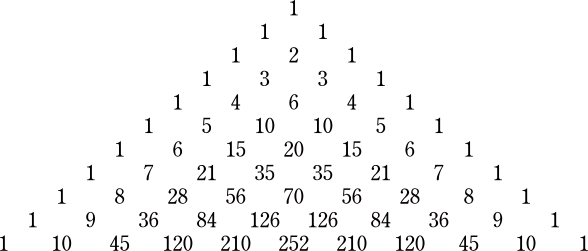
\includegraphics[width=\textwidth]{images/pascal_traingle.png}
\vspace{30px}

Пусть T (n, k) - k-й в нумерации с нуля элемент n-й строки. Свойства:
\begin{itemize}
    \item $T(n, k) = {n \choose k}$
    \item Симметричность строк: T(n, k) = T(n, n - k), n - строка, k - столбец.
    \item Возрастание чисел в первой половине строки: $T(n, i) \leqslant T (n, i + 1), 0 \leqslant i < n/2, i \in Z$
    \item $\sum_{k=0}^{n} T(n, k) = 2^n$
    \item $\sum_{k=0}^{n} (-1)^k T(n, k) = 0, n \neq 0$
\end{itemize}

\noindent
\textit{Рекуррентная соотношение} - последовательность, в которой каждый следующий член выражается через предыдущие элементы и, возможно, номер элемента.

\noindent
\textit{Рекуррентная формула} - формула вида $a_{n}=f(n,a_{n-1},a_{n-2},\dots ,a_{n-p})$, выражающая каждый член последовательности $a_{n}$ через p предыдущих членов и возможно номер члена последовательности n.

\parag{19. Образы и прообразы множеств. Полный прообраз.}
Пусть функция f из множества A в множество B устанавливает соответствие между элементами множеств A и B. Пусть $X \subseteq A$ – подмножество множества A. Функция f сопоставляет ему \textit{образ} $f(X) \subseteq B$ подмножества X. По определению f(X) состоит в точности из тех
элементов множества B, которые являются значениями элементов из X. Используя введённые нами для множеств обозначения, это можно записать как
\[
    f(X) = \{ b | \exists x \in X: b = f(x) \}
\]
Совокупность всех тех элементов $a \in A$, образом которых является данный элемент $b = f(a)$, $f(a) \in B$ , называется \textit{прообразом} элемента $b$ и обозначается $f^{-1}(b)$

\noindent
Подмножеству $Y \subseteq B$ можно сопоставить \textit{полный прообраз} $f^{-1}(Y) \subseteq A $ подмножества Y. По определению $f^{-1}(Y)$ состоит в точности из тех элементов A, значения которых лежат в Y. Или формально:
\[
    f^{-1}(Y) = \{a | f(a) \in Y\}
\]

\parag{20. Отображения (всюду определённые функции). Инъекции, сюръекции и биекции.}
Отображение множества A в множество B - функция, которому \underline{каждому} элементу $a \in A$ ставит в соответствие элемент $b \in B$.

\noindent
Пусть $f: A \to B$. Тогда функция f называется:

1) \textit{Инъективной (или инъекцией)}, если:
\[
    (b = f(a_{1}))\ \&\ (b = f(a_{2})) \Rightarrow (a_{1} = a_{2})
\]

2) \textit{Сюрьективной (или сюрьекцией)}, если:
\[
    \forall b \in B\ \exists a \in A: b = f(a)
\]

3) \textit{Биективной (или биекцией)}, если \textit{она сюрьективна и инъективна}. Биекции также называют \textit{взаимно-однозначными функциями}. 

\parag{21. Бинарные отношения. Транзитивность, симметричность, рефлексивность.}
\textit{Бинарным отношением между множествами A и B} называется подмножество R произведения $A \times B$. В том случае, когда A = B, мы говорим просто об отношении R на A.

Для бинарных отношений часто используется инфиксная форма записи:
\[
    aRb \overset{Def}{=} (a, b) \in R \subset A \times B 
\]

Пусть $R \subset A^{2}$. Тогда отношение R называется:

\begin{center}
\begin{tabular}{cc}
    \textit{рефлексивным}, & если $\forall a \in A\ (aRa)$ \\
    \textit{антирефликсивным}, & если $\forall a \in A\ \neg(aRa)$ \\
    \textit{симметричным}, & если $\forall a, b \in A\ (aRb \Rightarrow bRa)$ \\
    \textit{антисимметричным}, & если $\forall a, b \in A\ (aRb\ \&\ bRa \Rightarrow a = b)$ \\
    \textit{транзитивным}, & если $\forall a, b, c \in A\ (aRb\ \&\ bRc \Rightarrow aRc)$ \\
    \textit{линейным}, & если $\forall a, b \in A\ (a = b \lor aRb \lor bRa)$
\end{tabular}
\end{center}

\parag{22. Теоретико-множественные операции с отношениями. Операция обращения.}
Бинарные отношения — это множества пар элементов, связанных этими отношениями, поэтому к отношениям применимы все операции, выполняемые над множествами. Пусть $P \subseteq A \times A$ и $Q \subseteq A \times A$, тогда:

1) Пересечение отношений $P \cap Q$ - отношение, которое содержит только те упорядоченные пары, которые есть и в P и в Q:
\[
    P \cap Q = \{(x, y)\ |\ (x, y) \in P \land (x, y) \in Q\}
\]

2) Объединение отношений $P \cup Q$ - отношение, которое содержит все упорядоченные пары отношения P и все упорядоченные пары отношения Q:
\[
    P \cup Q = \{(x, y)\ |\ (x, y) \in P \lor (x, y) \in Q\}
\]

3) Разность отношений $P \setminus Q$ - отношение, которое содержит только те упорядоченные пары, которые содержатся в P, но не содержатся в Q:
\[
    P \setminus Q = \{(x, y)\ |\ (x, y) \in P \land (x, y) \notin Q\}
\]

4) Симметрическая разность отношений $P \bigtriangleup Q$ - отношение, которое содержит только те упорядоченные пары, которые содержатся в объединении P и Q, но не содержатся в пересечении P и Q:
\[
    P \bigtriangleup Q = \{(x, y)\ |\ (x, y) \in (P \cup Q) \land (x, y) \notin (P \cap Q)\}
\]

5) Дополнение отношения P - это отношение, состоящее из всех пар $(x, y) \in (A \times A)$, которые не входят в отношение P:
\[
    \bar P = \{(x, y)\ |\ (x, y) \in (A \times A) \land (x, y) \notin P\}
\]

6) Обратным отношением $P^{-1}$ к P называется такое отношение, которое содержит пару (x, y) тогда и только тогда, когда P содержит пару (y, x):
\[
    P^{-1} = \{(x, y)\ |\ (y, x) \in P\}
\]

\parag{23. Композиция бинарных отношений}
Пусть $R_{1} \subset A \times C$ - отношение между A и С, а $R_{2} \subset C \times B$ - отношение между C и B. \textit{Композицией} двух отношений $R_{1}$ и $R_{2}$ называется отношение $R \subset A \times B$ между A и B, определяемое следующим образом:
\[
    R \overset{Def}{=} R_{1} \circ R_{2} \overset{Def}{=} \{(a, b)\ |\ a \in A\ \&\ b \in B\ \&\ \exists c \in C\ (aR_{1}c\ \&\ cR_{2}b)\}
\]
Другими словами, $aR_{1} \circ R_{2}b \iff \exists c \in C\ (aR_{1}c\ \&\ cR_{2}b)$.

\parag{24. Отношения эквивалентности.}
Отношение на некотором множестве, которое одновременно рефлексивно, симметрично и транзитивно, называют \textit{отношением эквивалентности}.

\noindent
\textit{Классы эквивалентности} - непересекающиеся подмножества множества X, при этом любые два элемента одного класса находятся в
отношении R, а любые два элемента разных классов не находятся в отношении R.

\parag{25. Графы. Основные определения: ребра, вершины, степени вершин.}
Граф $G$ - совокупность двух множеств - непустого множества V (множества вершин) и множества E двухэлементных подмножеств множества V (E - множество ребер).
\[
    E = \{ \{u, v\}\ |\ u, v \in V, u \neq v \}
\]
\textit{Степень вершины $u$} - количество вершин, смежных с $u$. Обозначение: $d(u)$.

\parag{26. Пути и циклы в графах.}
\textit{Путь} - последовательность вершин $v_{1}, v_{2}, ..., v_{n}$, такая что $\forall i \in \{1, 2, ..., n - 1\}$: $v_{i}$ и $v_{i+1}$ - соединены ребром.


\noindent
\textit{Простой путь} - путь, такой что в нем все вершины различны.

\noindent
\textit{Цикл} - путь, такой что $v_{1} = v_{n}$

\noindent
\textit{Простой цикл} - цикл, все вершины которого, кроме первой и последней различны.

\parag{27. Отношение достижимости (связанности) и компоненты связности графа.}
Говорят, что вершина $v$ достижима из вершины $u$, если существует путь $v_{1}, v_{2}, ..., v_{n}$, где $v_{1} = u$, а $v_{n} = v$.
Связность вершины $u$ и $v$ означает их достижимость друг из друга.

\noindent
Обозначение связности: $u \rightarrow v$

\noindent
Основные свойства:

1) $u \rightarrow u\ \forall u \in V$

2) если $u \rightarrow v$, то $v \rightarrow u$ (для неор.графов)

3) Транзитивность (для неор.графов): если  $u \rightarrow v$ и  $v \rightarrow w$, то  $u \rightarrow w$

\noindent
\textit{Компонента связности} - подмножество множества вершин V графа G такое, что любая пара вершин в этом подмножестве связаны, а также любая вершина этого подмножества не связана с любой другой не из этого подмножества.

\noindent
\textit{Компонента связности} - класс эквивалентности по отношению достижимости (валидно, т.к. отношение достижимости является отношением эквивалентности, это следует из свойств).

\parag{28. Правильные раскраски графов. Формулировка критерия 2 - раскрашиваемости}
Раскраска вершин графа называется правильной, если концы каждого ребра покрашены в разные цвета. \textit{2-раскрашиваемые графы} - это графы, которые можно правильно раскрасить в 2 цвета. Граф 2-раскрашиваемый, когда в нем нет циклов нечетной длины. 

\noindent
Теорема. 2 - раскраска описанного типа возможна тогда и только тогда, когда в графе нет циклов нечётной длины.

\parag{29. Двудольные графы. Двудольные и двураскрашиваемые графы.}
Граф G(V, E) называется \textit{двудольным}, если множество V может быть разбито на два непересекающихся множества $V_{1}$ и $V_{2}$ ($V_{1} \cup V_{2} = V, V_{1} \cap V_{2} = \varnothing$), причем всякое ребро из E инцидентно вершине из $V_{1}$ и вершине из $V_{2}$ (соединяет вершину из $V_{1}$ с вершиной из $V_{2}$). Множества $V_{1}$ и $V_{2}$ называются \textit{долями} двудольного графа.

\noindent
\textit{2-раскрашиваемые графы} - это графы, которые можно правильно раскрасить в 2 цвета. Граф является 2-раскрашиваемым тогда и только тогда, когда является двудольным.

\parag{30. Подграфы. Изоморфизм графов. Клики и независимые множества.}
Граф $G'(V', E')$ называется \textit{подграфом} графа G(V, E), если $V' \subset V\ \&\ E' \subset E$.

\noindent
\textit{Изоморфизм графов.}
Говорят, что два графа, $G_{1}(V_{1}, E_{1})$ и $G_{2}(V_{2}, E_{2})$, \textit{изоморфны}, если существует биекция $h: V_{1} \rightarrow V_{2}$, такая что две вершины $u$ и $v$ графа $G_{1}$ смежны тогда и только тогда, когда вершины $h(u)$ и $h(v)$ смежны в графе $G_{2}$.


\noindent
\textit{Кликой} называется такое подмножество вершин графа, каждая пара которых связана ребром.

\noindent
\textit{Независимым множеством} называется такое подмножество вершин графа, никакая пара которых не связана ребром.


\parag{31. Эйлеровы циклы.}
Цикл называется \textit{эйлеровым}, если он проходит по всем рёбрам графа, причём только один раз.

\noindent
Критерии существования. Эйлеров цикл существует в неориентированном графе тогда и только тогда когда выполнены условия:

1) Граф связен.

2) Все вершины имеют четную степень.

3) Цикл проходит через все ребра.

\noindent
Эйлеров цикл существует в ориентированном графе тогда и только тогда когда выполнены условия:

1) Граф сильно связен.

2) Для любой вершины v верно $d^{-}(v) = d^{+}(v)$


\parag{32. Деревья. Полные бинарные деревья.}
\textit{Дерево} - связный граф без простых циклов длины $\geqslant$ 3. Для деревьев  выполняются эти свойства:

1) G - связный граф, где нельзя удалить ни одного ребра без нарушения связности.

2) G - связный граф, где число рёбер на единицу меньше числа вершин.

3) G - связный граф, где для любых двух вершин u, v существует единственный простой путь из u в v.

4) G - cвязный граф, где нет простых циклов длины больше 2.

(Все 4 определения эквиваленты)

\vskip 0.2in

\noindent
Еще свойства деревьев:

1) Для любых трёх вершин дерева, пути между парами этих вершин имеют ровно одну общую вершину. 

2) Из любого связного неориентированном графа можно получить дерево удалением части ребер. (Полученное дерево будет называться остовным деревом исходного графа). 

3) В любом дереве есть висячая вершина.

\vskip 0.2in

\noindent
\textit{Полное бинарное дерево глубины n} — неориентированный граф-дерево, вершины которого — двоичные слова длины не больше n, а рёбра соединяют слова, которые можно получить друг из друга добавлением (или исключением соответственно) символа в конец слова. Корень дерева — пустое слово.


\parag{33. Ориентированные графы, основные определения.}
\textit{Ориентированный граф (орграф)} - такой граф, в котором направление ребра имеет значение; ребра (v, u) и (u, v) - разные. Записать можно следующим образом: $E = \{(A, B), (C, D), ...\}$. Часто ребра в орграфе называют \textit{дугами}. 

\noindent
Для орграфов и неорграфов верно, что $u \rightarrow v$, $v \rightarrow w \Rightarrow u \rightarrow w$. 

\noindent
Для ориентированных графов отличают входящую степень $d^{-}(v)$ — количество входящих в вершину ребер, то есть ребер вида (u, v), и исходящую степень $d^{+}(v)$ — количество исходящих ребер, то есть ребер вида (v, u).

\noindent
Путь, простой путь, цикл, простой цикл - эквивалентно определениям для неорграфа.

\parag{34. Компоненты сильной связности ориентированного графа.}
Будем говорить, что вершины u и v сильно связны, когда $u \rightarrow v$ и $v \rightarrow u$. Обозначается как $u \leftrightarrow v$.

\noindent
\textit{Компонента сильной связности} — определено только для орграфов; аналогично обычной компоненте связности, но между любой парой вершин в компоненте должна быть сильная связность. 

\noindent
Теорема: Вершины ориентированного графа можно однозначно разбить на непересекающиеся группы, называемые сильно связными компонентами, при этом:

1) Каждая вершина графа попадает ровно в одну группу;

2) Любые две вершины из одной группы сильно связаны;

3) Любые две вершины из двух разных групп не являются сильно связанными (в одну из сторон — или даже в обе — пути нет).

\parag{35. Отношения частичного порядка (строгие и нестрогие), линейные порядки}
\textit{Отношение порядка} - антисимметричное транзитивное отношение.

\noindent
\textit{Нестрогое отношение порядка} - рефлексивное отношение порядка.

\noindent
\textit{Строгое отношение порядка} - антирефлексивное отношение порядка.

\noindent
\textit{Линейное отношение порядка} - отношение порядка, обладающее свойством линейности ($\forall a, b \in A\ (a = b \lor aRb \lor bRa)$).

\noindent
\textit{Частичное отношение порядка} - отношение порядка, не обладающее свойством линейности.

\vskip 0.2 em

Обычно отношение строгого порядка (линейного или частичного) обозначается знаком $\prec$, а отношение нестрогого порядка - знаком $\preceq$.

\parag{36. Отношение непосредственного следования}
\textit{Отношение непосредственного следования} - это отношение порядка $\prec$, такое что если $x < y$, то $\nexists z: x < z \land z < y$. Кратко записывается так:
\[
    \prec = \{(x, y)\ |\ (x < y) \land \neg(\exists z: x < z \land z < y)\}
\]

\parag{37. Изоморфные отношения частичного порядка}
Отношения частичного порядка $R_{1} \subseteq A \times A$ и $R_{2} \subseteq B \times B$ называются изоморфными, если существует такая биекция $f : A \rightarrow B$, что для $\forall x, y$ $xR_{1}y \iff f(x)R_{2}f(y)$

\vskip 2em
\section{Теоремы с доказательствами}

\parag{1. Разложение в ДНФ булевой функции.}
\textbf{Теорема:} Любая булева функция представима в виде дизъюнкции конъюнктов её переменных и может быть записана так:
\[
    f(x_{1}, ..., x_{n}) = \underset{\{(\sigma_{1}, ..., \sigma_{n})\ |\ f(\sigma_{1}, ..., \sigma_{n}) = 1\}}{\bigvee} x_{1}^{\sigma_{1}} \wedge x_{2}^{\sigma_{2}} \wedge ... \wedge x_{n}^{\sigma_{n}}
\]
\textbf{Замечание:} запись $x^{\sigma}$ означает буквально:
\[
    x^{\sigma} = \left\{
                    \begin{array}{ll}
                        x, \sigma = 1\\
                        \bar x, \sigma = 0
                    \end{array}
                \right.
\]

\vskip 1em

\noindent
Для того, чтобы доказать данную теорему, докажем теорему о разложении булевой функции по k переменным.

\noindent
\textbf{Теорема:} о разложении булевой функции по переменным.
\[
    f(x_{1}, ..., x_{m}, x_{m+1}, ..., x_{n}) = \underset{(\sigma_{1},  ..., \sigma_{m})}{\bigvee} x_{1}^{\sigma_{1}}\wedge...\wedge x_{m}^{\sigma_{m}} \wedge f(\sigma_{1}, ..., \sigma_{m}, x_{m+1}, ..., x_{n})
\]
Причем дизъюнкция берется по всем возможным наборам $(\sigma_{1}, ..., \sigma_{m}) \in \{0, 1\}^{m}$.

\noindent
\textbf{Доказательство:} Рассмотрим значение формулы на наборе значений $(a_{1}, ..., a_{n})$. Имеем:
\[
    \Big(\underset{(\sigma_{1},  ..., \sigma_{m})}{\bigvee} x_{1}^{\sigma_{1}}\wedge...\wedge x_{m}^{\sigma_{m}} \wedge f(\sigma_{1}, ..., \sigma_{m}, x_{m+1}, ..., x_{n})\Big)(a_{1}, ..., a_{n}) = 
\]
\[
    = \underset{(\sigma_{1},  ..., \sigma_{m})}{\bigvee} a_{1}^{\sigma_{1}}\wedge...\wedge a_{m}^{\sigma_{m}} \wedge f(\sigma_{1}, ..., \sigma_{m}, a_{m+1}, ..., a_{n})
\]
Достаточно очевидно, что $a^{\sigma} = 1$, если $a = \sigma$, иначе $a^{\sigma} = 0$:

\begin{center}
    \begin{tabular}{|c|c|c|}
        \hline
        a & $\sigma$ & $a^{\sigma}$  \\
        \hline
        0 & 0 & 1  \\
         \hline
        0 & 1 & 0  \\
        \hline
        1 & 0 & 0 \\
        \hline
        1 & 1 & 1 \\
        \hline
    \end{tabular}
\end{center}

\noindent
Следовательно, все конъюнкции, в которых $\exists i: a_{i} \neq \sigma_{i}$, равны 0 и их можно опустить, поэтому остается только одно слагаемое, для которого $\forall i \in \{1, ..., n\}\ (a_{i} = \sigma_{i})$. Следовательно:
\[
    \underset{(\sigma_{1},  ..., \sigma_{m})}{\bigvee} a_{1}^{\sigma_{1}}\wedge...\wedge a_{m}^{\sigma_{m}} \wedge f(\sigma_{1}, ..., \sigma_{m}, a_{m+1}, ..., a_{n}) = 
\]
\[
    = a_{1}^{a_{1}}\wedge...\wedge a_{m}^{a_{m}} \wedge f(a_{1}, ..., a_{m}, a_{m+1}, ..., a_{n}) = f(a_{1}, a_{2}, ..., a_{n})
\]
$\blacksquare$

Веренмся к первоначальной задаче. Достаточно очевидно, что искомое разложение в ДНФ - это разложение функции по всем переменным, m = n. (При таком разложении полностью исчезает часть с f(...)).

\vskip 5em
\parag{2. Обощенный закон Моргана.}
\[ \neg(x_{1} \vee x_{2} \vee ... \vee x_{n}) = \neg x_{1} \wedge \neg x_{2} \wedge ... \wedge \neg x_{n} \]
\[ \neg(x_{1} \wedge x_{2} \wedge ... \wedge x_{n}) = \neg x_{1} \vee \neg x_{2} \vee ... \vee \neg x_{n} \]

\noindent
Доказательство (для первой формулы, анналогично для второй):

\begin{enumerate}
    \item База: Выражение верно для n = 2: $\neg(x_{1}  \vee x_{2}) = \neg x_{1} \wedge \neg x_{2}$
    \item Предположение: Пусть верно для n = k - 1: \[ \neg(x_{1} \vee x_{2} \vee ... \vee x_{k - 1}) = \neg x_{1} \wedge \neg x_{2} \wedge ... \wedge \neg x_{k - 1} \]
    \item Шаг: проверим для n = k. Сделаем замену $y = x_{1} \vee x_{2} \vee ... \vee x_{k - 1}$
        $$ \neg(x_{1} \vee x_{2} \vee ... \vee x_{k}) = \neg(y \vee x_{k}) = \neg y \wedge \neg x_{k} = \neg (x_{1} \vee x_{2} \vee ... \vee x_{k - 1}) \wedge \neg x_{k} = $$
        $$= \neg x_{1} \wedge \neg x_{2} \wedge ... \wedge \neg x_{k - 1} \wedge \neg x_{k}$$
        
        (Последний переход выполнен по предположению индукции)
\end{enumerate}  

\parag{3. Формула включений и исключений.}
\textbf{Теорема:}
\[
    \Big|\underset{i = 1}{\overset{n}{\bigcup}}A_{i}\ \ \Big| =
    \underset{i=1}{\overset{n}{\sum}}|A_{i}| -
    \underset{1 \leqslant i < j \leqslant n}{\sum} |A_{i} \cap A_{j}|+
    ... +
    (-1)^{n-1} |A_{1} \cap ... \cap A_{n}|
\]
Доказательство (по индукции):

1) База индукции: докажите по диаграммам Эйлера-Венна для n = 2, 3

2) Предположение индукции: пусть верно для n - 1
\[
    \Big|\underset{i = 1}{\overset{n - 1}{\bigcup}}A_{i}\ \ \Big| =
    \underset{i=1}{\overset{n - 1}{\sum}}|A_{i}| -
    \underset{1 \leqslant i < j \leqslant n - 1}{\sum} |A_{i} \cap A_{j}|+
    ... +
    (-1)^{n-2} |A_{1} \cap ... \cap A_{n-1}|
\]

Дальше, нужно заметить, что из-за того, что операция пересечения ассоциативна по операции объединения, то верно вот что:

\[
    \Big(\overset{n-1}{\underset{i=1}{\bigcup}}A_{i}\Big) \cap A_{n} =
    \overset{n-1}{\underset{i=1}{\bigcup}}(A_{i} \cap A_{n})
\]

Кроме того, надо заметить, что для штуки, которую мы получили, верно предположение индукции (мы можем её разложить):

\[
    \Big|\underset{i = 1}{\overset{n - 1}{\bigcup}}(A_{i} \cap A_{n})\ \ \Big| =
    \underset{i=1}{\overset{n - 1}{\sum}}|A_{i} \cap A_{n}| -
    \underset{1 \leqslant i < j \leqslant n - 1}{\sum} |A_{i} \cap A_{j} \cap A_{n}|+
    ... +
    (-1)^{n-2} |A_{1} \cap ... \cap A_{n-1} \cap A_{n}|
\]

3) А теперь, зная все формулы выше, мы делаем шаг индукции:

\[
    \Big|\underset{i = 1}{\overset{n}{\bigcup}}A_{i}\ \ \Big| =\
    \Big|\Big(\underset{i = 1}{\overset{n - 1}{\bigcup}}A_{i}\Big)\cup A_{n}\ \ \Big|
\]

По формуле для n = 2 раскрываем эту скобку:
\[
    \Big|\Big(\underset{i = 1}{\overset{n - 1}{\bigcup}}A_{i}\Big)\cup A_{n}\ \ \Big| =
    \Big|\underset{i = 1}{\overset{n-1}{\bigcup}}A_{i}\ \ \Big| +
    |A_{n}| -\ 
    \Big|\Big(\overset{n-1}{\underset{i=1}{\bigcup}}A_{i}\Big) \cap A_{n}\ \Big| =
\]
\[
    = \Big|\underset{i = 1}{\overset{n-1}{\bigcup}}A_{i}\ \ \Big| +
    |A_{n}| -\ 
    \Big|\overset{n-1}{\underset{i=1}{\bigcup}}(A_{i} \cap A_{n})\ \Big| =
\]
\[
    \Bigg( \underset{i=1}{\overset{n - 1}{\sum}}|A_{i}| -
    \underset{1 \leqslant i < j \leqslant n - 1}{\sum} |A_{i} \cap A_{j}|+
    ... +
    (-1)^{n-2} |A_{1} \cap ... \cap A_{n-1}| \Bigg) + |A_{n}| -
\]
\[
    - \Bigg( \underset{i=1}{\overset{n - 1}{\sum}}|A_{i} \cap A_{n}| -
    \underset{1 \leqslant i < j \leqslant n - 1}{\sum} |A_{i} \cap A_{j}|+
    ... +
    (-1)^{n-2} |A_{1} \cap ... \cap A_{n-1} \cap A_{n}| \Bigg) =
\]
\[
    \Big(\underset{i=1}{\overset{n - 1}{\sum}}|A_{i}| + |A_{n}| \Big) -
    \Bigg( \underset{1 \leqslant i < j \leqslant n - 1}{\sum} |A_{i} \cap A_{j}| +  \underset{i=1}{\overset{n - 1}{\sum}}|A_{i} \cap A_{n}| \Bigg) + ... -
\]
\[
    -(-1)^{n-2} |A_{1} \cap ... \cap A_{n-1} \cap A_{n}| = \underset{i=1}{\overset{n}{\sum}}|A_{i}| -
    \underset{1 \leqslant i < j \leqslant n}{\sum} |A_{i} \cap A_{j}|+
    ... +
    (-1)^{n-1} |A_{1} \cap ... \cap A_{n}|
\]
$\blacksquare$

\parag{4.Число k-элементных подмножеств n-элементного множества есть ${n \choose k}$}
Будем выбирать элементы множества по очереди. Первый элемент можно выбрать n способами, второй (n - 1) способами (годятся все, кроме первого, уже выбранного), третьий (n - 2) способами, и т.д пока не выберем k элементов. По правилу произведения всего способов выбрать таким образом есть
\[
    n \times (n - 1) \times (n - 2) \times ... \times (n - k + 1)
\]
способ. Однако так мы посчитали не число возможных подмножеств, а число упорядоченных списков. Получается, нужно не обращать внимания на позицию элемента в списке. Всего можно составить k! таких упорядоченных списков из k элементов (k! - количество способов переставить элементы в списке). Значит количество способов выбрать k-элементное подмножество из n-элементного множества равно 
\[
    \frac{n(n-1)(n-2)\cdot...\cdot(n-k+1)}{k!} =
    \frac{n(n-1)(n-2)\cdot...\cdot2\cdot1}{(n-k)(n-k-1)\cdot...\cdot2\cdot1} \times \frac{1}{k!} = 
\]
\[
    = \frac{n!}{(n-k)!} \times \frac{1}{k!} = \frac{n!}{(n-k)!\cdot k!} = {n \choose k}
\]
$\blacksquare$

\parag{5. Бином Ньютона. Формула для биномиальных коэффициентов.}
\textbf{Теорема:}
\[
    (a + b)^{n} = \overset{n}{\underset{k=0}{\sum}} {n \choose k} a^{n - k}b^{k}
\]
\textit{Доказательство (по индукции):}

1) База индукции: n = 1
\[
    (a + b)^{1} = a + b = a^{1}b^{0} + a^{0}b^{1} = {1 \choose 0} a^{1}b^{0} + {1 \choose 1}a^{0}b^{1} = 
    \underset{k=0}{\overset{1}{\sum}} {1 \choose k} a^{1-k}b^{k}
\]

2) Пусть верно для n:
\[
    (a + b)^{n} = \overset{n}{\underset{k=0}{\sum}} {n \choose k} a^{n- k}b^{k}
\]

3) Докажем для n + 1:
\[
    (a + b)^{n+1} = (a + b)(a + b)^{n} = (a + b) \Big(\overset{n}{\underset{k=0}{\sum}} {n \choose k} a^{n- k}b^{k}\Big) = 
\]
\[
    a\times \Big( \overset{n}{\underset{k=0}{\sum}} {n \choose k} a^{n- k}b^{k}\Big) + b \times \Big(\overset{n}{\underset{k=0}{\sum}} {n \choose k} a^{n- k}b^{k}\Big) = 
\]
\[
    = \Big( \overset{n}{\underset{k=0}{\sum}} {n \choose k} a^{n - k + 1}b^{k}\Big) + \Big( \overset{n}{\underset{k=0}{\sum}} {n \choose k} a^{n-k}b^{k + 1}\Big)
\]
Вынесем из первой скобки одно слагаемое при k = 0, а из второй скобки слагаемое при k = n:
\[
    \Big( \overset{n}{\underset{k=0}{\sum}} {n \choose k} a^{n - k + 1}b^{k}\Big) + \Big( \overset{n}{\underset{k=0}{\sum}} {n \choose k} a^{n-k}b^{k + 1}\Big) =
\]
\[
    = a^{n+1} + \Big( \overset{n}{\underset{k=1}{\sum}} {n \choose k} a^{n - k + 1}b^{k}\Big) + b^{n+1} + \Big( \overset{n-1}{\underset{k=0}{\sum}} {n \choose k} a^{n-k}b^{k + 1}\Big)
\]
Сделаем сдвиг в сумме во второй скобке. Будем проходиться не от 0 до n - 1, а от 1 до n. Тогда, чтобы сумма осталась неизменной нужно из всех k под знаком суммы отнять единчку. Получаем:
\[
    a^{n+1} + \Big( \overset{n}{\underset{k=1}{\sum}} {n \choose k} a^{n - k + 1}b^{k}\Big) + b^{n+1} + \Big( \overset{n-1}{\underset{k=0}{\sum}} {n \choose k} a^{n-k}b^{k + 1}\Big) =
\]
\[
    = a^{n+1} + \Big( \overset{n}{\underset{k=1}{\sum}} {n \choose k} a^{n - k + 1}b^{k}\Big) + b^{n+1} + \Big( \overset{n}{\underset{k=1}{\sum}} {n \choose k - 1} a^{n-(k-1)}b^{k}\Big) = 
\]
\[
    = a^{n+1} + b^{n+1} + \Big( \overset{n}{\underset{k=1}{\sum}} {n \choose k} a^{n - k + 1}b^{k}\Big) + \Big( \overset{n}{\underset{k=1}{\sum}} {n \choose k - 1} a^{n-k+1}b^{k}\Big) =
\]
\[
    = a^{n+1} + b^{n+1} +  \overset{n}{\underset{k=1}{\sum}} \Big({n \choose k} a^{n - k + 1}b^{k} + {n \choose k - 1} a^{n-k+1}b^{k}\Big) =
\]
\[
    =  a^{n+1} + b^{n+1} +  \overset{n}{\underset{k=1}{\sum}} \Big( a^{n - k + 1}b^{k} \big( {n \choose k - 1} + {n \choose k} \big)\Big) =
\]
\[
    =  a^{n+1} + b^{n+1} +  \overset{n}{\underset{k=1}{\sum}} \Big( a^{n - k + 1}b^{k} \times {n + 1 \choose k}\Big) =
\]
\[
    = a^{n+1} + \overset{n}{\underset{k=1}{\sum}} {n + 1 \choose k} a^{n - k + 1}b^{k} + b^{n+1} = 
    \overset{n + 1}{\underset{k=0}{\sum}} {n + 1 \choose k} a^{(n+1)- k}b^{k}
\]
$\blacksquare$

\parag{6. Основные свойства треугольника Паскаля: симметричность строк, возрастание чисел в первой половине строки.}
1) ${n \choose k} = {n \choose n - k}$, следовательно все строки треугольника Паскаля симметричны. (доказывается раскрытием обоих частей).

\noindent
2) Решить неравенство ${n \choose k} < {n \choose k + 1}$. Получаем, что оно выполняется только при $k \leqslant \frac{n}{2}$. Из симметричности получаем возрастание в первой половине строки и убывание во второй половине строки.

\parag{7. Основные свойства треугольника Паскаля: формула для суммы чисел в строке, нижняя оценка на центральный коэффициент}
\textbf{Теорема 1:} Сумма чисел в n-ой строке треугольника Паскаля = $2^{n}$.
\vskip 1em

\noindent
\textit{Доказательство:}
Вспомним, что в n-ой строке треугольника Паскаля лежат числа
\[
    {n \choose 0} + {n \choose 1} + ... + {n \choose n} =
    {n \choose 0} 1^{0}1^{n - 0} + {n \choose 1} 1^{1}1^{n - 1} + ... + {n \choose n} 1^{n}1^{n - n} =
\]
\[
    = \underset{k=0}{\overset{n}{\sum}} {n \choose k} 1^{n -k}1^{k} =
    (1 + 1)^{n} = 2^{n}
\]

\vskip 2em
\noindent
\textbf{Теорема 2:} Нижняя оценка на центральный коэффициент.
\[
    {2n \choose n} \geqslant \frac{2^{2n}}{2n+1}
\]

\vskip 1em
\noindent
\textit{Доказательство:}

1) Рассмотрим сумму 2n-ой строки треугольника Паскаля:
\[
    {2n \choose 0} + {2n \choose 1} + ... + {2n \choose 2n} = 2^{2n}
\]

2) Из возрастания биномальных коэффициентов следует, что:
\[
    {2n \choose n} \geqslant {2n \choose k}, \forall k \in \{1, 2, ..., 2n\} 
\]

3) Следовательно:
\[
    \underbrace{{2n \choose n} + ... + {2n \choose n}}_{2n + 1} \geqslant {2n \choose 0} + {2n \choose 1} + ... + {2n \choose 2n}
\]

4) Тогда:
\[
    (2n + 1) {2n \choose n} \geqslant {2n \choose 0} + {2n \choose 1} + ... + {2n \choose 2n}
\]

5) Получаем:
\[
    (2n + 1) {2n \choose n} \geqslant 2^{2n}
\]

6) И наконец:
\[
    {2n \choose n} \geqslant \frac{2^{2n}}{2n + 1}
\]

\noindent
$\blacksquare$

\parag{8. Число решений уравнения $x_{1} + x_{2} + ... + x_{k} = n$ в неотрицательных целых числах. (Задача Муавра.)}
Есть ещё одна задача, где естественным (но не вполне очевидным) образом возникают числа сочетаний. Сколько решений имеет уравнение $x_{1} + x_{2} + ... + x_{k} = n$ в целых неотрицательных числах? Если это недостаточно наглядно, можно спросить иначе: есть k различных человек и n одинаковых монет. Сколькими способами можно раздать этим людям эти монеты? Каждый такой способ определяется тем, сколько монет получил каждый (но какие именно монеты — не учитывается, все монеты одинаковые). Это целые неотрицательные числа (допускаются варианты, где некоторые получили по нулю монет). Как найти это число? Представим себе, что наши n монет разложены в ряд. Прежде чем раздавать эти монеты, разделим их на k групп перегородками, и договоримся, кому идёт самая левая группа, кому вторая слева и т.д. Заметим, что мы допускаем случай, когда две перегородки оказываются рядом — это значит просто, что человеку, которому была назначена группа между ними, не повезло и в этом раскладе ему ни одной монеты не достанется. Каждому варианту раздачи (каждому решению уравнения в неотрицательных числах) соответствует последовательность из n монет и k - 1 перегородок. (Число перегородок на единицу меньше числа группы: первая группа стоит слева от первой перегородки, а последняя - справа от последней.) Наоборот, каждой последовательности из n монет и k - 1 перегородок соответствует некоторый способ раздачи монет. Поэтому надо подсчитать число способов расставить перегородки. А это совсем просто - каждый содержащее n монет и k - 1 перегородок. Это количество, как мы знаем, равно ${n + k - 1 \choose n}$ или ${n + k - 1 \choose k - 1}$.

\parag{9. Основная теорема об отношениях эквивалентности (классы эквивалентности на множестве A — в точности разбиения множества A на подмножества)}
\textbf{Теорема:} Любое отношение R, являющееся отношением эквивалентности на множестве A, делит A на классы эквивалентности - непересекающиеся подмножества множества X, при этом любые два элемента одного класса находятся в отношении R, а любые два элемента разных классов не находятся в отношении R.

\vskip 1em

\noindent
\textit{Доказательство:} Для каждого $x \in A$ рассмотрим множество тех y, для которых верно $R(x, y)$.
Обозначим его через [x]. Его можно было бы назвать «классом эквивалентности элемента x» - собственно говоря, так его и называют, но само по себе это название не гарантирует разбиения на классы, это ещё надо доказывать. А именно, надодоказать, что
\begin{enumerate}
    \item объединение всех множеств вида [x] совпадает с множеством A;
    \item два множества [x] и [y] либо не пересекаются, либо совпадают;
    \item наконец, надо ещё доказать, что [x] = [y] в том и только том случае, когда R(x, y), то есть R совпадает с отношением «принадлежать одному классу».
\end{enumerate}
По порядку:
\begin{enumerate}
    \item В силу рефлексивности множество [x] содержит x в качестве своего элемента: $x \in [x]$, поскольку R(x, x). Отсюда следует, что объединение всех этих множеств совпадает с A. (Выйти за пределы A они не могут, так как мы рассматриваем отношение на множестве A и элементы множества A.)
    \item Пусть для двух элементов $x, y \in A$ их классы [x] и [y] пересеклись. Это означает, что есть такой $z \in A$, что R(x, z) и R(y, z). Симметричность даёт R(z, y), после чего мы применяем транзитивность к R(x, z) и R(z, y) и заключаем, что R(x, y). Выведем отсюда, что [x] = [y]. В самом деле, если произвольный элемент t принадлежит [y], то R(y, t). Вспоминая, что R(x, y)и применяя транзитивность, получаем R(x, t), то есть $t \in [x]$. Мы доказали, таким образом, что $[y] \subseteq [x]$. Аналогично доказывается, что $[x] \subseteq [y]$, так что [x] = [y].
    \item Если для каких-то x, y верно R(x, y), то x и y оба лежат в одном классе, а именно, в [x]. Обратно, если x и y лежат в каком-то [z], то по определению имеем R(z, x) и R(z, y), симметричность даёт R(x, z) и после этого транзитивность даёт R(x, y).
\end{enumerate}

\parag{10. Нижняя оценка числа связных компонент в неориентированном графе.}
\textbf{Теорема:} Число компонент связности в графе не меньше, чем разность количества вершин и ребер.

\vskip 1em

\noindent
\textit{Доказательство (по индукции):}

1) База индукции (n = 1): граф состоит из 1 вершины, которая является единственной компонентой связности в графе. Разность количества вершин(1) и ребер(0) равно 1, но компонента связности одна. База доказана.

2) Шаг индукции $(n \mapsto n + 1)$: пусть для всех графов на n вершинах выполняется эта оценка, добавим еще одну вершину и рассмотрим случай связи, при котором сумма количества компонент связности и количество ребер наименьшая: выберем такой граф на n вершинах (C - количество компонент связности в этом графе, E - количество ребер в этом графе), чтобы в нем эта сумма была наименьшей и добавим к нему еще одну вершину. Заметим, что если связать новую вершину хотя бы одним ребром с k уже существовавшими компонентами связности, то количество ребер увеличится, как минимум, на k, а компонент связности станет на k - 1 меньше, чем в графе на n вершинах. (Если не связывать, то станет на одну больше, так как будет еще одна компонента связности, если связать компоненты связности, то они станут одной компонентой связности, то есть количество уменьшится на единицу.) Так как нужна наименьшая сумма, то нужно использовать, как можно меньше ребер: будем соединять вершину 1 ребром с каждой из k существовавших компонентов связности - ребер станет на k больше, а количество компонентов связности уменьшится на k - 1, то есть сумма компонентов связности и ребер нового графа будет такой: (C - (k - 1)) + (E + k) = C + E + 1. Но C + E + 1 > V + 1 из C + E > V. Значит для n + 1 верна оценка.

\noindent
$\blacksquare$

\parag{11. Доказательство критерия 2-раскрашиваемости неориентированного графа.}
\textbf{Формулировка:} Раскраска вершин графа в два цвета так, чтобы рёбра соединяли вершины разных цветов, возможна когда и только тогда, когда в графе нет циклов нечётной длины.

\vskip 1em

\noindent
\textit{Доказательство:} Если в графе есть цикл нечётной длины, то его нельзя раскрасить: соседние вершины должны быть противоположных цветов, и дойдя до конца, мы получим противоречие. Чтобы доказать обратное, предположим, что циклов нечётной длины нет. Выберем некоторую вершину $a$ и не ограничивая общности окрасим её в цвет 1. Для любой другой вершины $b$ посмотрим, сколько рёбер в пути от $a$ к $b$. Заметим, что если есть путь $a \rightarrow b$ с чётным числом рёбер, а также другой путь $a \rightarrow b$ с нечётным числом рёбер, то есть цикл с нечётным числом рёбер (из $a$ в $b$ по одному пути и из $b$ в $a$ - по другому). Это противоречит предположению. Таким образом, мы поделили вершины графа на два типа: соединённые с $a$ путями чётной длины и путями нечётной длины. Если какая-то вершина соединена с $a$ путями чётной длины, то её соседи соединены путями нечётной длины (один такой путь - через соседа - заведомо есть, а тогда и все пути имеют нечётную длину). Раскрасим те, что на чётном расстоянии в то же цвет, что и $a$, а те, что на нечётном - в другой. Требуемая раскраска одной компоненты связности построена. Остальные можно раскрашивать совершенно независимо от этой, так как нет ребёр, которые могли бы помешать.

\noindent
$\blacksquare$

\parag{12. 13. 14. Я не знаю, как это ддоказывать по отдельности. Они еще напихали только те переходы, которых нет в книжке, это было спланировано. Поэтому буду пытаться, если что, доказывать эквивалентность всего.}
\textbf{Теорема:} Все четыре указанных свойства равносильны: граф, обладающий одним из них, обладает и всеми остальными

1) Cвязный граф, где нельзя удалить ни одного ребра без нарушения связности.

2) Cвязный граф, где число рёбер на единицу меньше числа вершин.

3) Cвязный граф, где для любых двух вершин u, v существует единственный простой путь из u в v.

4) Cвязный граф, где нет простых циклов длины больше 2.

\noindent
\textit{Доказательство:}

\noindent
$(2) \Rightarrow (1)$. Если в графе число рёбер на единицу меньше числа вершин, то после удаления ребра их будет на 2 меньше, а мы уже знаем, что в этом случае связность нарушится.

\noindent
$(1) \Rightarrow (2)$. Пусть дан связный граф с n вершинами, в котором ни одного ребра нельзя удалить без нарушения связности. Как мы доказывали, что в нём не меньше n-1 рёбер? Мы представляли себе, что рёбра добавляются по очереди, и смотрели, как меняется число связных компонент. Если добавленное ребро соединяло вершины, которые уже и так связаны, число компонент не менялось; в противном случае оно уменьшалось на единицу. Теперь первый случай невозможен: в нём добавленное ребро соединяет то, что соединено и так (другими рёбрами), поэтому оно лишнее и в окончательном графе (его можно удалить без нарушения связности, вопреки предположению). Поэтому к моменту, когда останется одна компонента, было добавлено как раз V - 1 рёбер, где V - число вершин.

\noindent
Итак, (1) и (2) равносильны. Теперь докажем, что из этих свойств следует (3), то есть единственность простых путей. Здесь снова нужно будет смотреть за процессом добавления рёбер - мы знаем, что добавляемое ребро всегда соединяет две разные компоненты - и по индукции доказывать, что нет двух простых путей с одинаковыми началом и концом.

\noindent
Итак, предположим, что это свойство выполнено для графа из нескольких связных компонент, и мы добавляем туда ребро p–q, соединяя две различные компоненты P и Q (содержащие p и q соответственно). Нам надо доказать, что и для нового графа это свойство выполнено. Пусть это не так, и есть два простых пути с одинаковым началом u и одинаковым концом v. Как минимум один из этих путей должен включать новое ребро p–q, поскольку до его добавления свойство единственности выполнялось (предположение индукции). Ребро это может входить только один раз, поскольку путь простой. Значит, начало пути лежит в одной из компонент P или Q, а конец в другой (остальные рёбра старые и не переводят в другую компоненту). Пусть, например, u лежит в P, а v лежит в Q. Тогда путь состоит из трёх частей: простой путь от u до p, ребро p–q, и простой путь от v до q. Посмотрим теперь на другой путь из u в v и убедимся, что он совпадает с первым. Он тоже должен использовать ребро p–q, поскольку перед добавлением этого ребра вершины u и v лежали в разных компонентах. Тогда по тем же причинам он разбивается на часть от u до p, ребро p–q, и часть от q до v. Остаётся воспользоваться предположением индукции (единственность пути в старом графе от u до p, и от q до v) и увидеть, что два рассматриваемых пути совпадают.

\noindent
Из (3) легко следует (4). В самом деле, если есть простой цикл $a_{1} \leftrightarrow a_{2} \leftrightarrow ...  a_{n} \leftrightarrow a_{1}$, где n > 2 и все $a_{1}, ..., a_{n}$ различны, то есть два простых пути из $a_{1}$ в $a_{n}$, а именно путь $a_{1} \leftrightarrow a_{2} \leftrightarrow ... \leftrightarrow a_{n}$ и путь из одного ребра $a_{1} \leftrightarrow a_{n}$.

\noindent
Наконец, надо убедиться, что из (4) следует (1) и (2). Снова нужно вспомнить процесс слияния компонент при добавлении рёбер. Если (1) и (2) неверны, то в какой-то момент добавляется ребро, соединяющее уже связанные друг с другом вершины. Эти вершины связаны простым путём (как мы доказали), и вместе с добавленным ребром получится цикл. При этом длина цикла по крайней мере 3, потому что имевшийся простой путь был с пересадками (ребра-то раньше не было).

\noindent
Теорема об эквивалентности четырёх свойств доказана

\noindent
$\blacksquare$

\parag{15. Равносильность свойств ориентированных графов: (1) каждая компонента сильной связности со- стоит из одной вершины; (2) вершины графа возможно занумеровать так, чтобы каждое ребро вело из вершины с меньшим номером в вершину с большим номером; (3) в графе нет циклов длины больше 1.}
\textbf{Теорема: } Следующие свойства ориентированного графа равносильны:
\begin{enumerate}
    \item Каждая сильно связная компонента состоит из одной вершины.
    \item В графе нет циклов длины больше 1.
    \item Вершины графа возможно занумеровать так, чтобы каждое ребро вело из вершины с меньшим номером в вершину с большим номером.
\end{enumerate}

\vskip 1em
\noindent
\textit{Доказательство:}
Начнём с очевидных утверждений. Если в графе есть цикл с n > 1 вершинами, то вершины этого цикла сильно связаны (из любой можно попасть в любую по циклу), так что из первого свойства следует второе. Наоборот, если различные вершины a, b сильно связаны, то существуют пути из $a$ в $b$ и из $b$ в $a$,
и из этих двух путей можно составить цикл. Наконец, если возможна нумерация
вершин, при которой рёбра ведут от вершин с меньшим номером к вершинам с большим, то цикла нет: вдоль него номера вершин должны расти, и вернуться в начало мы не сможем. 
Осталось доказать единственное нетривиальное утверждение: если в ориентированном графе нет циклов, то его вершины можно пронумеровать требуемым способом.

\noindent
\textbf{Лемма}. В ориентированном графе без циклов есть вершина, из которой не выходит ни одного ребра.

\noindent
\textit{Доказательство леммы:} Пусть это не так и из любой вершины выходит хоть одно ребро. Возьмём какую-то вершину $a_{1}$, из неё идёт ребро в какую-то другую вершину $a_{2}$, из неё идёт ребро ещё куда-то, и так далее. Поскольку граф конечен, то рано или поздно мы придём второй раз в какую-то вершину $a_{i}$, где уже были, и участок пути после $a_{i}$ свернётся в цикл - вопреки предположению, что циклов нет.

\noindent
Теперь можно закончить доказательство теоремы. Выберем вершину, из которой
не ведёт ни одного ребра. Ей можно без опаски присвоить номер, больший всех
остальных номеров. Поэтому рассуждаем по индукции: удалив эту вершину (и все
входящие в неё рёбра) из графа, получим граф без циклов. (Циклы в нём были бы циклами и в исходном графе.) Пронумеруем его вершины от 1 до какого-то числа n (число оставшихся вершин) с соблюдением условия (рёбра ведут из меньшего к большему), и после этого вернём выброшенную вершину под номером n + 1. (Базис индукции — граф с одной вершиной — очевиден.)

\noindent
$\blacksquare$

\parag{16. Критерий существования эйлерова цикла в неориентированном графе.}
\textbf{Теорема:} Неориентированный граф без вершин нулевой степени содержит эйлеров цикл тогда и только тогда, когда он связен и степени всех вершин чётны.

\vskip 1em
\noindent
\textit{Доказательство:} Пусть в графе эйлеров цикл есть. Тогда он проходит через все вершины (поскольку они имеют ненулевую степень), и по нему можно дойти от любой вершины до любой. Значит, граф связен. Теперь про степени. Возьмём какую-то вершину v, пусть она встречается в цикле k раз. Идя по циклу, мы приходим в неё k раз и уходим k раз, значит, использовали
k входящих и k исходящих рёбер. При этом, раз цикл эйлеров, других рёбер у этой вершины нет, так что в графе её степень равна 2k. Таким образом, в одну
сторону критерий доказан.

\noindent
В обратную сторону. Будем рассматривать пути, которые не проходят дважды по одному ребру. (Таков, например, путь из одного ребра.) Выберем среди них самый длинный путь
\[
    a_{1} \rightarrow a_{2} \rightarrow a_{3} \rightarrow ... \rightarrow
    a_{n-1} \rightarrow a_{n}
\]
и покажем, что он является искомым циклом, то есть что $a_{1} = a_{n}$ и что он содержит все рёбра. В самом деле, если он самый длинный, то добавить к нему ребро $a_{n} \rightarrow a_{n+1}$ уже нельзя, то есть все выходящие из an рёбра уже использованы. Это возможно, лишь если $a_{1} = a_{n}$. В самом деле, если вершина $a_{n}$ встречалась только внутри пути (пусть она входит k раз внутри пути и ещё раз в конце пути), то мы использовали k + 1 входящих рёбер и k выходящих, и больше выходящих нет. Это противоречит чётности степени.

\noindent
Итак, мы имеем цикл, и осталось доказать, что в него входят все рёбра. В самом деле, если во всех вершинах цикла использованы все рёбра, то из вершин этого цикла нельзя попасть в вершины, не принадлежащие циклу, то есть использованы все вершины (мы предполагаем, что граф связен или сильно связен) и, следовательно, все рёбра. С другой стороны, если из какой-то вершины $a_{i}$ выходит ребро $a_{i} \rightarrow v$,
то путь можно удлинить до
\[
    a_{i} \rightarrow a_{i+1} \rightarrow ... \rightarrow a_{n} = a_{1} \rightarrow a_{2} \rightarrow ... \rightarrow a_{i} \rightarrow v
\]
вопреки нашему выбору (самого длинного пути). Аналогично можно получить противоречие и для входящего ребра $v \rightarrow a_{i}$, добавив его в начало. (А можно заметить, что если есть неиспользованное входящее ребро, то есть и неиспользованное выходящее.) Это рассуждение было для ориентированного случая, но в неориентированном всё аналогично. Теорема доказана.

\noindent
$\blacksquare$

\parag{17.Критерий обратимости остатка (вычета) по модулю N.}
\textbf{Теорема:} Число $a$ обратимо по модулю $p$, если $a$ и $p$ взаимно просты, то есть их наибольший общий делитель равен единице.

\vskip 1em
\noindent
\textit{Доказательство:}

1) Пусть НОД(a, p) = d, $d > 1$. Заметим, что $1 < d < p$, так как делитель не может быть больше самого числа.

2) Раз d - наибольший общий делитель $a$ и $p$, то существуют $k_{1}, k_{2}$ такие что:
\[ a = k_{1} \cdot d \]
\[ p = k_{2} \cdot d \]

3) Тогда $a \cdot k_{2}$ сравнимо с нулём по модулю p, т.к:
\[
    a \cdot k_{2} \equiv k_{1} \cdot k_{2} \cdot d \equiv k_{1} \cdot p \equiv 0\ (mod\ p)
\]

4) Обратимость числа $a$ значит, что $\exists a^{-1}$, такое что:
\[
    a \cdot a^{-1} \equiv 1\ (mod\ p)
\]

5) Кроме того, имеем: $a \cdot k_{2} \equiv 0\ (mod\ p)$. Домножим обе части уравнения в пункте 4 на $k_{2}$:
\[
    k_{2} \cdot a \cdot a^{-1} \equiv k_{2}\ (mod\ p)  
\]

6) Получаем:
\[
    0 \cdot a^{-1} \equiv k_{2}\ (mod\ p)
\]
\[
    0 \equiv k_{2}\ (mod\ p)
\]

7) Получили противоречние. Следовательно, $\not\exists a^{-1}$, который удовлетворяет этим условиям, если $a$ и $p$ не взаимно просты. Тогда исходная теорема доказана по принципу контрапозиции.

\vskip 1em
\noindent
$\blacksquare$

\parag{18. Малая теорема Ферма.}
\textbf{Теорема:} Если $p$ — простое число и $a$ — целое число, не делящееся на $p$, то $a^{p-1} \equiv 1\ (mod\ p)$.

\vskip 1em
\noindent
\textit{Доказательство:}

\begin{enumerate}
    \item Пусть $f(x) = x^{p}$. Докажем, что $\forall x\ f(x) = x\ (mod\ p)$.
    \item Докажем это: 
    \begin{enumerate}
        \item $f(0) \equiv 0^{p} \equiv 0\ (mod\ p)$
        \item $f(1) \equiv 1^{p} \equiv 1\ (mod\ p)$
        \item $\forall x, y \notin \{0, 1\}\ f(x + y) \equiv$ \[
            \equiv (x + y)^{p} \equiv
            x^{p} + {p \choose 1} x^{p-1}y^{1} + ... + {p \choose p - 1} x^{1}y^{p-1} + y^{p} \equiv
        \]
        \[
            \equiv x^{p} + \frac{p!}{1!(p-1)!}x^{p-1}y^{1} + ... + \frac{p!}{(p-1)!1!}x^{1}y^{p-1} + y^{p} \equiv
        \]
        \[
            \equiv x^{p} + y^{p} \equiv f(x) + f(y)\ (mod\ p)
        \]
        \item Т.к $f(x + y) \equiv f(x) + f(y)\ (mod\ p)$, то мы можем вычислить f для всех остальных x:
        \begin{enumerate}
            \item $f(2) \equiv f(1) + f(1) \equiv 1 + 1 \equiv 2\ (mod\ p)$
            \item $f(3) \equiv f(2 + 1) \equiv f(2) + f(1) \equiv 2 + 1 \equiv 3\ (mod\ p)$
            \item ...
            \item $f(x) \equiv f((x - 1) + 1) \equiv x - 1 + 1 \equiv x\ (mod\ p)$
        \end{enumerate}
    \end{enumerate}
    
    \item Получаем, что $f(a) \equiv a^{p} \equiv a\ (mod\ p)$
    \item Число $p$ - простое, поэтому все остатки по модулю $p$ взаимно просты с $p \Rightarrow \forall x\ \exists x^{-1}: x \cdot x^{-1} \equiv 1\ (mod\ p)$ (по критерию обратимости).
    
    \item Следовательно, $\exists a^{-1}: a^{-1} \cdot a \equiv 1\ (mod\ p)$
    
    \item \textit{Тогда используя эту лемму:} "Если $a \equiv b\ (mod\ m)$ и $c \equiv d\ (mod\ m)$, то $ac \equiv bd\ (mod\ m)$", получаем:
    \begin{equation*}
        \begin{cases}
            a^{p} \equiv a\ (mod\ p) \\
            a^{-1} \equiv a^{-1}\ (mod\ p)
        \end{cases}
        \begin{matrix}
            \Rightarrow\ \ a^{p-1} \equiv 1\ (mod\ p)
        \end{matrix}
    \end{equation*}
    
\end{enumerate}

\noindent
$\blacksquare$

\end{document}
